\section{Probes}

To observe the system under test, the resulting outcomes, the result of causal links and outcome expressions, we must put probes in the system. 

For each outcome of interest, a probe (observation point) is attached to measure the delay of the outcome, like one would in a true oscilloscope. 

These probes allow to connect the system under test to the stub, which in turns sends outcome instances to the oscilloscope, which performs statistical computations on all the time series. 

Consider the figure below, a probe is attached at every component to measure the delay of N outcome ($p_2, p_3$), the stub will send the outcome instance data for each probe observing an outcome to the oscilloscope, which will measure their respective $\Delta$Qs from the time series data and display them (if chosen by the user). 

Another probe ($p_1$) is inserted at the beginning and end of the system to measure the global execution delay. 

Thanks to this probe, the user can observe the $\Delta$Q \textit{"observed at $p_1$"}, which is the $\Delta$Q which was calculated from the data received by inserting probe $p_1$. The \textit{$\Delta$Q "calculated at $p_1$"} is the resulting $\Delta$Q from the convolution of the observed $\Delta$Qs at $c_2$ and $c_3$.   
    \begin{figure}[H]
        \begin{center}
            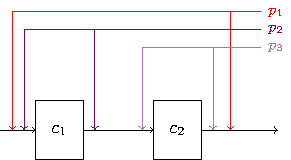
\includegraphics[scale=1.8]{tikz/probes.pdf}
        \end{center}
        \label{fig:probes}
        \caption{Probes inserted in a component diagram.}
    \end{figure}

    \subsection{Inserting probes in the oscilloscope}
        Probes are automatically inserted in the oscilloscope when defining outcomes, part of the system the user wishes to observe and operators. 
        
        In the system below, which is equal to the one defined above, probes are automatically attached to outcomes $o_1, o_2$. The user who wants to observe the result of the sequential composition can insert probes at the start and end of the routine. 

        \begin{figure}[H]
            \begin{center}
                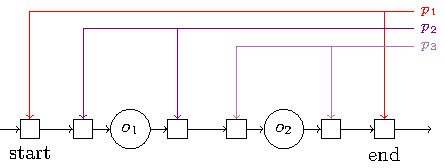
\includegraphics[scale=1.3]{tikz/probe_1.pdf}
            \end{center}
            \label{fig:probes_o}
            \caption{Probes inserted in the outcome diagram of the previous component diagram. \ref{fig:probes}}
        \end{figure}
       
       As for operators (outcome expression), probes are automatically attached to the components inside them and to the start event and end events of the operators. 

       \begin{figure}[H]
           \begin{center}
                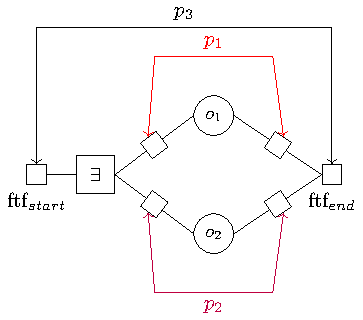
\includegraphics[scale = 1.3]{tikz/probe_2.pdf}
            \end{center}
            \label{fig:probes_op}
            \caption{Probes inserted into an operator.}
       \end{figure}
    
    The \textbf{observed $\Delta$Q} for the first-to-finish operator is the $\Delta$Q from the instances (\textbf{start}, \textbf{end}). The \textbf{calculated $\Delta$Q} is the $\Delta$Q which is the result of the first-to-finish operator being applied on $o_1, o_2$
        
    \subsection{Probes: from spans to outcome instances}
        OpenTelemetry spans are useful to carry context, attributes and baggage in a program, the plethora of attributes they have is nevertheless too much for the oscilloscope.

        To get the equivalent of spans for the oscilloscope, the stub needs to be called at the starting events of a probe to start an instance, and at the ending events to end the outcome instance and send the data to the oscilloscope.

        \begin{minted}{erlang}
        % Start the outcome instance of worker_2 
        {WorkerCtx, WorkerPid} = otel_wrapper:start_span(<<"worker_2">>),
        
        % Do work here ...

        %End the outcome instance of worker_2
        otel_wrapper:end_span(WorkerCtx, WorkerPid),
        \end{minted}
